%%%%%%%%%%%%%%%%%%%%%%%%%%%%%%%%%%%%%%%%%
% Beamer Presentation
% LaTeX Template
% Version 1.0 (10/11/12)
%
% This template has been downloaded from:
% http://www.LaTeXTemplates.com
%
% License:
% CC BY-NC-SA 3.0 (http://creativecommons.org/licenses/by-nc-sa/3.0/)
%
%%%%%%%%%%%%%%%%%%%%%%%%%%%%%%%%%%%%%%%%%

%----------------------------------------------------------------------------------------
%	PACKAGES AND THEMES
%----------------------------------------------------------------------------------------

\documentclass[serif,mathserif,professionalfont]{beamer}

\mode<presentation> {

% The Beamer class comes with a number of default slide themes
% which change the colors and layouts of slides. Below this is a list
% of all the themes, uncomment each in turn to see what they look like.

%\usetheme{default}
%\usetheme{AnnArbor}
%\usetheme{Antibes}
%\usetheme{Bergen}
%\usetheme{Berkeley}
%\usetheme{Berlin}
%\usetheme{Boadilla}
%\usetheme{CambridgeUS}
%\usetheme{Copenhagen}
%\usetheme{Darmstadt}
%\usetheme{Dresden}
%\usetheme{Frankfurt}
%\usetheme{Goettingen}
%\usetheme{Hannover}
%\usetheme{Ilmenau}
%\usetheme{JuanLesPins}
%\usetheme{Luebeck}
\usetheme{Madrid}
%\usetheme{Malmoe}
%\usetheme{Marburg}
%\usetheme{Montpellier}
%\usetheme{PaloAlto}
%\usetheme{Pittsburgh}
%\usetheme{Rochester}
%\usetheme{Singapore}
%\usetheme{Szeged}
%\usetheme{Warsaw}

% As well as themes, the Beamer class has a number of color themes
% for any slide theme. Uncomment each of these in turn to see how it
% changes the colors of your current slide theme.

%\usecolortheme{albatross}
%\usecolortheme{beaver}
%\usecolortheme{beetle}
%\usecolortheme{crane}
%\usecolortheme{dolphin}
%\usecolortheme{dove}
%\usecolortheme{fly}
%\usecolortheme{lily}
%\usecolortheme{orchid}
%\usecolortheme{rose}
%\usecolortheme{seagull}
%\usecolortheme{seahorse}
%\usecolortheme{whale}
%\usecolortheme{wolverine}

%\setbeamertemplate{footline} % To remove the footer line in all slides uncomment this line
%\setbeamertemplate{footline}[page number] % To replace the footer line in all slides with a simple slide count uncomment this line

%\setbeamertemplate{navigation symbols}{} % To remove the navigation symbols from the bottom of all slides uncomment this line
}

\usepackage{graphicx} % Allows including images
\usepackage{booktabs} % Allows the use of \toprule, \midrule and \bottomrule in tables

\newcommand{\norm}[1]{\left\lVert #1 \right\rVert}

\usepackage{amsmath}
\usepackage{amssymb}
\usepackage{bm}
\usepackage{multirow}
\usepackage{pxfonts}
\usepackage{eulervm}

%----------------------------------------------------------------------------------------
%	TITLE PAGE
%----------------------------------------------------------------------------------------

\title[Section for EN.553.413/613]{Section for Applied Statistics and Data Analysis} % The short title appears at the bottom of every slide, the full title is only on the title page

\author{TA: Cong Mu} % Your name
\institute[cmu2@jhu.edu] % Your institution as it will appear on the bottom of every slide, may be shorthand to save space
{
Office Hour: Wednesday 10:00AM - 12:00PM
%Johns Hopkins University \\ % Your institution for the title page
\medskip
\textit{} % Your email address
}
\date{November 22, 2019} % Date, can be changed to a custom date

\begin{document}

\begin{frame}
\titlepage % Print the title page as the first slide
\end{frame}

\begin{frame}
\frametitle{Overview} % Table of contents slide, comment this block out to remove it
\tableofcontents % Throughout your presentation, if you choose to use \section{} and \subsection{} commands, these will automatically be printed on this slide as an overview of your presentation
\end{frame}

%----------------------------------------------------------------------------------------
%	PRESENTATION SLIDES
%----------------------------------------------------------------------------------------

%------------------------------------------------
% Sections can be created in order to organize your presentation into discrete blocks, all sections and subsections are automatically printed in the table of contents as an overview of the talk

% A subsection can be created just before a set of slides with a common theme to further break down your presentation into chunks
%------------------------------------------------

\section{Some Statistics}


%    	\begin{figure}
%    		\includegraphics[width=1\linewidth]{figure1}
%    	\end{figure}
%	
%    	\vspace{0.5cm}
%    	
%    	\rightline{{\tiny (Figure from Linear Models with R)}}
	
%	\begin{block}{Claim}
%		The marginal distributions of bivariate normal $ \mathcal{N}(\mu_X, \mu_Y, \sigma_X^2, \sigma_Y^2, \rho) $ are normal with
%		$$ f_X (x) = \int_{- \infty}^{\infty} f_{X,Y}(x, y) dy = \frac{1}{\sigma_X \sqrt{2 \pi}} \exp \left[- \frac{(x-\mu_X)^2}{2 \sigma_X^2} \right] $$
%		$$ f_Y (y) = \int_{- \infty}^{\infty} f_{X,Y}(x, y) dx = \frac{1}{\sigma_Y \sqrt{2 \pi}} \exp \left[- \frac{(y-\mu_Y)^2}{2 \sigma_Y^2} \right] $$
%	\end{block}




%\begin{frame}
%	
%	\frametitle{Review}
%	
%	\begin{block}{Recall}
%		For random variables $ X_1, X_2, \cdots, X_n $
%		$$ \mathbb{E} \left[\sum_{i=1}^{n} X_i \right] = \sum_{i=1}^{n} \mathbb{E}\left[X_i \right]. $$
%		$$ Var\left[\sum_{i=1}^{n} X_i  \right] = \sum_{i=1}^{n} Var \left[X_i \right] + \sum_{i \neq j} Cov \left[X_i, X_j \right]. $$
%	\end{block}
%	
%\end{frame}


%\begin{frame}
%	
%	\frametitle{Review}
%	
%	\begin{block}{Recall}
%		Given $ f_{X_1, X_2} (x_1, x_2) $ with $ Y_1 = g_1(X_1, X_2) $ and $ Y_2 = g_2(X_1, X_2) $ 
%		$$ f_{Y_1, Y_2}(y_1, y_2) = f_{X_1, X_2}(x_1, x_2) \; |J(x_1, x_2)|^{-1}. $$
%		where
%		\[
%		J(x_1, x_2) = 
%		\begin{vmatrix}
%		\frac{\partial g_1}{\partial x_1} & \frac{\partial g_1}{\partial x_2} \\
%		\frac{\partial g_2}{\partial x_1} & \frac{\partial g_2}{\partial x_2} \\
%		\end{vmatrix}
%		=
%		\frac{\partial g_1}{\partial x_1} \; \frac{\partial g_2}{\partial x_2} - \frac{\partial g_1}{\partial x_2} \; \frac{\partial g_2}{\partial x_1}
%		\]
%		and
%		$$ x_1 = h_1(y_1, y_2), \; x_2 = h_2(y_1, y_2) $$
%	\end{block}
%	
%\end{frame}


	



%\begin{frame}
%	
%	\frametitle{Properties of Least Squares Estimates}
%	
%	\begin{itemize}
%		\item General Formulation
%		$$ y = X \beta + \epsilon \qquad \text{where} \qquad \epsilon \sim  \mathcal{N}(0, \sigma^2 I) $$
%		\item Least Squares Estimates
%		$$ \widehat{\beta} = \left(X^\top X \right)^{-1} X^\top y. $$
%		\item Properties 
%		$$ \mathbb{E}\left[y\right] = X \beta, \qquad Var\left[y\right] = \sigma^2 I. $$
%		$$ \mathbb{E}\left[\widehat{\beta} \right] = \beta, \qquad Var\left[\widehat{\beta} \right] = \sigma^2 \left(X^\top X \right)^{-1}. $$
%	\end{itemize}
%
%	
%	
%\end{frame}




%\subsection{Confidence Intervals}
%
%
%
%\begin{frame}
%	
%	\frametitle{Confidence Intervals for Coefficients}
%	
%	\begin{itemize}
%		\item Recall
%		$$ Var\left[\widehat{\beta} \right] = \sigma^2 \left(X^\top X \right)^{-1}, \qquad \widehat{\sigma}^2 = s^2 = \frac{SSE}{n-p}. $$
%		\item General form
%		$$ \text{Estimate} \pm \text{Critical Value} \times \text{SE of Estimate}. $$
%		\item In particular, $ 100(1-\alpha)\% $ CI for $ \widehat{\beta}_i $
%		$$ \widehat{\beta}_i \pm t_{n-p}^{(\alpha/2)} \widehat{\sigma} \sqrt{\left(X^\top X \right)^{-1}_{ii}}. $$
%	\end{itemize}
%	
%	
%\end{frame}



%\begin{frame}
%	
%	\frametitle{Confidence Intervals for Predictions}
%	
%		\begin{itemize}
%		\item Recall
%		$$ \widehat{y}_0 = x_0^\top \widehat{\beta}, \qquad Var \left[\widehat{y}_0 \right] = \sigma^2 x_0^\top \left(X^\top X \right)^{-1} x_0 . $$
%		\item $ 100(1-\alpha)\% $ CI for a single future response
%		$$ \widehat{y}_0 \pm t_{n-p}^{(\alpha/2)} \widehat{\sigma} \sqrt{1 + x_0^\top \left(X^\top X \right)^{-1} x_0}. $$
%		\item $ 100(1-\alpha)\% $ CI for the mean response for given $ x_0 $
%		$$ \widehat{y}_0 \pm t_{n-p}^{(\alpha/2)} \widehat{\sigma} \sqrt{x_0^\top \left(X^\top X \right)^{-1} x_0}. $$
%	\end{itemize}
%	
%	
%\end{frame}





\subsection{Changes of Scale}




\begin{frame}
	
	\frametitle{Changes of Scale}
	
	\begin{itemize}
		\item A change of scale is often helpful when values of variables are all very large or all very small
		\begin{itemize}
			\item Interpretation
			\item Numerical stability
		\end{itemize}
		\item $ x_i \to \frac{x_i + a}{b} $
		\begin{itemize}
			\item t-statistic, F-statistic, $ R^2 $ and $ \widehat{\sigma}^2 $ unchanged
			\item $ \widehat{\beta}_i \to b \widehat{\beta}_i $
		\end{itemize}
		\item $ y \to \frac{y + a}{b} $
		\begin{itemize}
			\item t-statistic, F-statistic and $ R^2 $ unchanged
			\item $ \widehat{\beta} \to b \widehat{\beta} $, $ \widehat{\sigma} \to b \widehat{\sigma} $
		\end{itemize}
	\end{itemize}
	
	
	
\end{frame}



\subsection{Collinearity}




\begin{frame}
	
	\frametitle{Collinearity}
	
	\begin{itemize}
		\item Collinearity leads to imprecise estimates of $ \beta $
		\item Detection of collinearity
		\begin{itemize}
			\item Correlation matrix of the predictors
			\item Regression of $ x_i $ on all other predictors
			\item Eigenvalues of $ X^\top X $
			\item Variance inflation factor $ \frac{1}{1 - R_i^2} $
		\end{itemize}
	\end{itemize}
	
	
	
\end{frame}




\subsection{Weighted Least Squares}




\begin{frame}
	
	\frametitle{Weighted Least Squares}
	
	\begin{itemize}
		\item $ Var [\epsilon] = \sigma^2 I \to Var [\epsilon] = \sigma^2 \Sigma $
		\item \textbf{Generalized Least Squares} \newline
		The errors are dependent
		$$ \widehat{\beta} = \left(X^\top \Sigma^{-1} X \right)^{-1} X^\top \Sigma^{-1} y, \quad Var \left[\widehat{\beta} \right] = \sigma^2 \left(X^\top \Sigma^{-1} X \right)^{-1}. $$
		\item \textbf{Weighted Least Squares} \newline
		The errors are independent but not identically distributed
		$$ \Sigma = \text{diag}\left(\frac{1}{w_1}, \cdots, \frac{1}{w_n} \right). $$
	\end{itemize}
	
	
	
	
\end{frame}





%\begin{frame}
%	
%	\frametitle{Goodness of Fit}
%	
%	$$ SSTO = SSR + SSE, \qquad R^2 = \frac{SSR}{SSTO} = 1 - \frac{SSE}{SSTO} $$
%	where
%	$$ SSTO = \sum_{i=1}^{n} \left(y_i - \bar{y} \right)^2 $$
%	$$ SSR = \sum_{i=1}^{n} \left(\widehat{y}_i - \bar{y} \right)^2 $$
%	$$ SSE = \sum_{i=1}^{n} \left(y_i - \widehat{y}_i \right)^2 $$
%	
%\end{frame}

%\begin{frame}
%	
%	\frametitle{Inference in Regression}
%	
%	\begin{itemize}
%		\item Recall Sum of Squares Error
%		$$ SSE = \sum_{i=1}^{n} \left(y_i - \widehat{y}_i \right)^2 $$
%		\item Hypothesis Tests to Compare Models
%		$$ H_0: \text{Smaller Model} \;\; \omega \;\; \text{with dimension} \;\; q  $$
%		$$ H_A: \text{Larger Model} \;\; \Omega \;\; \text{with dimension} \;\; p $$
%%		$$ F = \frac{\left(SSE_{\omega} - SSE_{\Omega} \right) / \left(df_{\omega} - df_{\Omega} \right)}{SSE_{\Omega}/df_{\Omega}} = \frac{\left(SSE_{\omega} - SSE_{\Omega} \right) / \left(p-q \right)}{SSE_{\Omega}/(n-p)}  \sim F(p-q, n-p). $$
%		$$ F = \frac{\left(SSE_{\omega} - SSE_{\Omega} \right) / \left(p-q \right)}{SSE_{\Omega}/(n-p)}  \sim F(p-q, n-p). $$
%		$$ \text{Reject} \;\; H_0 \;\; \text{if} \;\; F > F_{\alpha}(p-q, n-p). $$
%	\end{itemize}
%
%	
%\end{frame}





%------------------------------------------------




%\begin{frame}
%	
%	\frametitle{Summary of Different Methods}
%	
%	\tiny
%	\begin{table}[H]
%		\centering
%		\begin{tabular}{|l|l|l|l|}
%			\hline
%			\textbf{Subspace Clustering Methods}                                                    & \textbf{Advantages}                                                                                                                                                                                                              & \textbf{Disadvantages}                                                                                                                          & \textbf{Assumption}                                                                                                                                                                       \\ \hline
%			\textbf{\begin{tabular}[c]{@{}l@{}}Local Subspace Affinity \\ (LSA)\end{tabular}}       & \multirow{2}{*}{\begin{tabular}[c]{@{}l@{}}1. Conceptually simple\\ 2. Computationally fast\\ 3. Robust against outliers \\     to some extent\end{tabular}}                                                                     & \begin{tabular}[c]{@{}l@{}}1. Only work in     \\ linear subspaces\\ 2. Inaccurate near \\ the intersection of \\ two subspaces\end{tabular}    & \multirow{2}{*}{\begin{tabular}[c]{@{}l@{}}The number of the nearest \\ neighbor needs to be small \\ enough and large enough\end{tabular}}                                               \\ \cline{1-1} \cline{3-3}
%			\textbf{\begin{tabular}[c]{@{}l@{}}Local Best Fit Flat \\ (SLBF)\end{tabular}}          &                                                                                                                                                                                                                                  & \begin{tabular}[c]{@{}l@{}}Inaccurate near \\ the intersection of \\ two subspaces\end{tabular}                                                 &                                                                                                                                                                                           \\ \hline
%			\textbf{\begin{tabular}[c]{@{}l@{}}Spectral Curvature Clustering \\ (SCC)\end{tabular}} & \begin{tabular}[c]{@{}l@{}}1. A better similarity \\ measure using points \\ from the entire data set\\ 2. Better justified \\ theoretically\\ 3. Can be extended to \\ nonlinear manifolds \\ using kernel methods\end{tabular} & \begin{tabular}[c]{@{}l@{}}Computational \\ complexity \\ would grow \\ exponentially \\ with the dimension \\ of the \\ subspaces\end{tabular} & \begin{tabular}[c]{@{}l@{}}1. A prior knowledge about \\ the subspace dimension might \\ be required\\ 2. The subspaces need to have \\ the same or very close \\ dimensions\end{tabular} \\ \hline
%			\textbf{\begin{tabular}[c]{@{}l@{}}Low-Rank Subspace Clustering \\ (LRSC)\end{tabular}} & \begin{tabular}[c]{@{}l@{}}1. Computational simplicity\\ 2. Closed form solution \\ with uncorrupted data or \\ data corrupted by noise\end{tabular}                                                                             & \begin{tabular}[c]{@{}l@{}}Few theoretical \\ justification\\ with corrupted data\end{tabular}                                                  & \begin{tabular}[c]{@{}l@{}}1. Uncorrupted data needs to \\ be drawn from independent \\ subspaces\\ 2. The union of subspaces \\ needs to be of low rank\end{tabular}                     \\ \hline
%			\textbf{\begin{tabular}[c]{@{}l@{}}Sparse Subspace Clustering \\ (SSC)\end{tabular}}    & \begin{tabular}[c]{@{}l@{}}Can recover a subspace \\ preserving representation \\ under much broader \\ conditions\end{tabular}                                                                                                  & \begin{tabular}[c]{@{}l@{}}No solution in \\ closed form\end{tabular}                                                                           & \begin{tabular}[c]{@{}l@{}}1. Subspaces need to be \\ sufficiently separated\\ 2. Data needs to be well \\ distributed inside the \\ subspaces\end{tabular}                               \\ \hline
%		\end{tabular}
%	\end{table}
%	
%	
%	
%\end{frame}






\section{Some Programming}


\subsection{Examples in Faraway}



\begin{frame}
	
	\frametitle{Examples in Faraway Chapter 7 \& 8}
	
	
	\begin{itemize}
		\item \textbf{Example:} \texttt{savings} dataset
		\item \textbf{Example:} \texttt{seatpos} dataset
		\item \textbf{Example:} \texttt{fpe} dataset
	\end{itemize}
	
	
	
\end{frame}













%------------------------------------------------


%\section{Covering Number Bound}


%------------------------------------------------

%\subsection{Covering Number}
%
%\begin{frame}
%	
%	\frametitle{Covering Number}
%	
%	\begin{definition}[Covering Number]
%		Let $ (A,d) $ be a metric space. For any $ \epsilon > 0 $, the covering number $ \mathcal{N} (A, \epsilon, d) $ of $ A $ with respect to $ d $ is the minimal $ k \in \mathbb{N} $ such that $ A $ can be covered with $ k $ balls of radius $ \epsilon $. i.e. 
%		$$ \forall a \in A, \quad \exists a_i \in \{a_1, . . . , a_k \} \subset A: \quad d(a, a_i) \le \epsilon . $$
%	\end{definition}
%    
%    \begin{columns}[c] % The "c" option specifies centered vertical alignment while the "t" option is used for top vertical alignment
%    	
%    	\column{.45\textwidth} % Left column and width
%    	\begin{figure}
%    		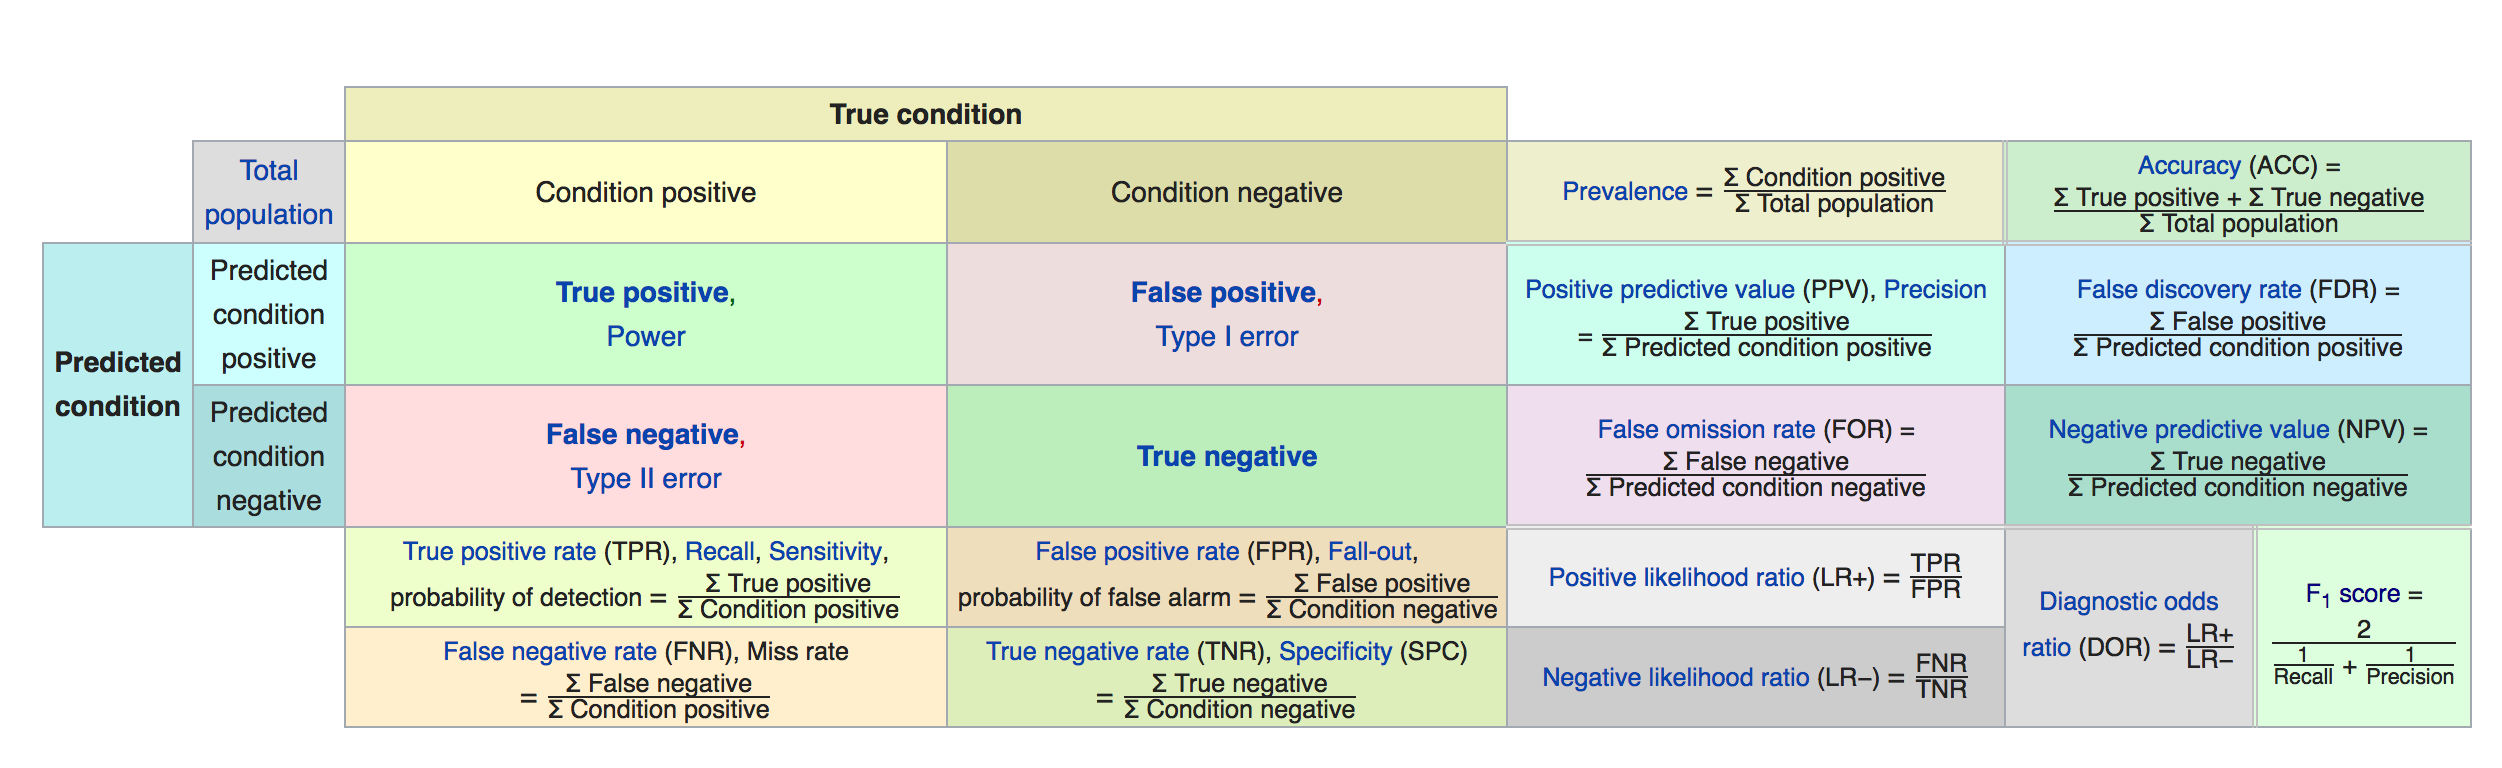
\includegraphics[width=0.7\linewidth]{p1}
%    	\end{figure}
%      
%    	
%    	\column{.5\textwidth} % Right column and width
%    	
%    	
%    	 A pentagon $ K $ is covered by seven balls of radius $ \epsilon $, which implies that $ \mathcal{N} (K, \epsilon, d) \le 7 $. 
%    	
%    	\vspace{0.5cm}
%    	
%    	 \rightline{{\tiny (Figure from High-Dimensional Probability)}}
%    	
%    \end{columns}
%
%
%\end{frame}





%------------------------------------------------

%\subsection{General Case}
%
%\begin{frame}
%	
%	\frametitle{Covering Number Bounds Rademacher Complexity}
%	
%	\begin{lemma}[]
%		Let $ c = \min_{\bar{\bm{a}}} \max_{\bm{a} \in A} ||\bm{a} - \bm{\bar{a}}|| $. Then for $ \forall M \in \mathbb{N}^+ $, with respect to $ L_2 $ norm, we have
%		$$ \widehat{\mathcal{R}}_S(A) \le \frac{c2^{-M}}{\sqrt{m}} + \frac{6c}{m} \sum_{k=1}^{M} 2^{-k} \sqrt{\log (\mathcal{N}(A,c2^{-k}, \ell_2))}. $$
%	\end{lemma}
%
%\end{frame}



%------------------------------------------------



%\begin{frame}
%	
%	\frametitle{Proof Outline}
%	
%	\begin{block}{Step 1}
%		Consider the set $ B_0 = \{ 0 \} $ and note that it is a $ c $-cover of $ A $. Let $ B_1, \cdots, B_M $ be sets such that each $ B_k $ corresponds to a minimal $ (c2^{-k}) $-cover of $ A $. Let $ \bm{a^*} = \arg \max_{\bm{a} \in A} <\bm{\sigma}, \bm{a}^*> $. For each $ k $, let $ \bm{b}^{(k)} $ be the nearest neighbor of $ \bm{a}^* $ in $ B_k $.  Then we show that
%		$$ || \bm{b}^{(k)} - \bm{b}^{(k-1)} || \le 3c 2^{-k}. $$
%	\end{block}
%	
%\end{frame}



%------------------------------------------------



%\begin{frame}
%	
%	\frametitle{Proof Outline}
%	
%	\begin{block}{Step 2}
%		Define $ \hat{B}_k = \{ (\bm{a} - \bm{a}^\prime): \bm{a} \in B_k, \bm{a}^\prime \in B_{k-1}, || \bm{a} - \bm{a}^\prime || \le 3c 2^{-k} \} $, we show that
%		$$ \widehat{\mathcal{R}}_S(A) \le \frac{1}{m} \mathbb{E}  \bigg[||\bm{\sigma}|| \  ||\bm{a}^* - \bm{b}^{(M)}|| \bigg] + \sum_{k=1}^{M} \frac{1}{m} \mathbb{E} \bigg[ \sup_{\bm{a} \in \hat{B}_k} <\bm{\sigma}, \bm{a}> \bigg]. $$
%	\end{block}
%
%	\begin{block}{Step 3}
%		Show that
%		$$ \frac{1}{m} \mathbb{E}  \bigg[||\bm{\sigma}|| \  ||\bm{a}^* - \bm{b}^{(M)}|| \bigg] \le \frac{c2^{-M}}{\sqrt{m}}, $$
%		$$ \frac{1}{m} \mathbb{E} \sup_{\bm{a} \in \hat{B}_k} <\bm{\sigma}, \bm{a}> \le \frac{6c 2^{-k} \sqrt{\log (\mathcal{N}(A, c2^{-k}, \ell_2))}}{m}. $$
%	\end{block}
%	
%\end{frame}




%------------------------------------------------



%\begin{frame}
%	
%	\frametitle{Covering Number Bound}
%	
%	\begin{theorem}[]
%		Let $ H $ be a family of functions mapping $ X $ to a subset of real numbers $ Y \subseteq \mathbb{R} $. Let $ D $ denote a distribution over $ X \times Y $. Let $ S = \{(x_i, y_i) \}_{i=1}^m $ denote i.i.d. sample drawn from $ D $. With respect to squared loss, we have
%		$$ R(h) = \mathbb{E}_{(x,y) \sim D} [(h(x)-y)^2], \quad \widehat{R}(h) = \frac{1}{m} \sum_{i=1}^{m} (h(x_i)-y_i)^2. $$
%		Assume that $ H $ is bounded, i.e. 
%		$$ \exists M > 0: \  |h(x) - y| \le M \quad \forall (x,y) \in X \times Y. $$ 
%		Then with respect to $ L_\infty $ norm we have 
%		$$ P_{S \sim D^m} \bigg[\sup_{h \in H} |R(h) - \widehat{R}(h)| \ge \epsilon \bigg] \le \mathcal{N} \bigg(H, \frac{\epsilon}{8M}, \ell_\infty \bigg) 2 \exp \bigg(\frac{-m \epsilon^2}{2M^4} \bigg). $$
%	\end{theorem}
%
%\end{frame}



%------------------------------------------------


%\begin{frame}
%	
%	\frametitle{Proof Outline}
%	
%	\begin{block}{Step 1}
%		Let $ L_S = R(h) - \widehat{R}(h) $, we show that for all $ h_1, h_2 \in H $ and any sample $ S $, the following holds:
%		$$ |L_S(h_1) - L_S(h_2)| \le 4M ||h_1 - h_2||_\infty = 4M \max_{x \in S} |h_1(x) - h_2(x)|. $$
%	\end{block}
%
%    \begin{block}{Step 2}
%    	Assume that $ H $ can be covered by $ k $ subsets $ B_1, \cdots, B_k $, i.e. $ H = B_1 \cup \cdots \cup B_k $. Then we show that for any $ \epsilon > 0 $, the following holds:
%    	$$ P_{S \sim D^m} \bigg[\sup_{h \in H} |L_S(h)| \ge \epsilon \bigg] \le \sum_{i=1}^{k} P_{S \sim D^m} \bigg[\sup_{h \in B_i} |L_S(h)| \ge \epsilon \bigg]. $$
%    \end{block}
%
%\end{frame}


%------------------------------------------------

%\begin{frame}
%	
%	\frametitle{Proof Outline}
%	
%	\begin{block}{Step 3}
%		Let $ k = \mathcal{N} \bigg(H, \frac{\epsilon}{8M}, \ell_\infty \bigg) $ and $ B_1, \cdots, B_k $ be 
%		balls of radius $ \frac{\epsilon}{8M} $ centered at $ h_1, \cdots, h_k $ covering $ H $. Use the result from Step 1, we show that for all $ i \in [1,k] $, the following holds:
%		$$ P_{S \sim D^m} \bigg[\sup_{h \in B_i} |L_S(h)| \ge \epsilon \bigg] \le P_{S \sim D^m} \bigg[ |L_S(h_i)| \ge \frac{\epsilon}{2} \bigg]. $$
%		Then by Hoeffding's inequality, we have
%		$$ P_{S \sim D^m} \bigg[ |L_S(h_i)| \ge \frac{\epsilon}{2} \bigg] \le 2 \exp \bigg(\frac{-m \epsilon^2}{2M^4} \bigg). $$
%	\end{block}
%
%\end{frame}


%------------------------------------------------

%\begin{frame}
%	
%	\frametitle{Proof Outline}
%	
%	\begin{block}{Step 4}
%		\begin{equation}
%		\begin{split}
%		P_{S \sim D^m} \bigg[\sup_{h \in H} |R(h) - \widehat{R}(h)| \ge \epsilon \bigg] & \le \sum_{i=1}^{k} P_{S \sim D^m} \bigg[\sup_{h \in B_i} |L_S(h)| \ge \epsilon \bigg] \\
%		& \le \sum_{i=1}^{k} P_{S \sim D^m} \bigg[ |L_S(h_i)| \ge \frac{\epsilon}{2} \bigg] \\
%		& \le \sum_{i=1}^{k} 2 \exp \bigg(\frac{-m \epsilon^2}{2M^4} \bigg) \\
%		& = \mathcal{N} \bigg(H, \frac{\epsilon}{8M}, \ell_\infty \bigg) 2 \exp \bigg(\frac{-m \epsilon^2}{2M^4} \bigg).
%		\nonumber
%		\end{split}
%		\end{equation}
%	\end{block}
%	
%\end{frame}



%------------------------------------------------

%\subsection{Linear Function Classes}

%------------------------------------------------



%\begin{frame}
%	
%	\frametitle{Linear Function Classes}
%	
%	\begin{lemma}[Maurey]
%		In a Hilbert space, let
%		$$ f = \sum_{j=1}^{d} w_j z_j \quad \text{and} \quad \alpha = \sum_{j=1}^{d} w_j \le 1, $$
%		where $ ||z_j|| \le L $, $ w_j \ge 0 $. Then for every $ m \ge 1 $, $ \exists b_1, \cdots, b_d \ge 0 $ such that
%		$$ \bigg|\bigg| f - \frac{1}{m} \sum_{j=1}^{d} b_j z_j \bigg|\bigg|^2 \le \frac{\alpha L^2 - ||f||^2}{m} \quad \text{and} \quad \beta = \sum_{j=1}^{d} b_j \le m. $$
%	\end{lemma}
%
%   
%\end{frame}



%------------------------------------------------


%\begin{frame}
%	
%	\frametitle{Covering Number Bound for Linear Function Classes}
%	
%	\begin{theorem}[]
%		Consider linear function classes below. If $ ||\bm{x}||_p \le L $, $ ||\bm{w}||_q \le B $, $ 2 \le p \le \infty $ and $ 1/p + 1/q = 1 $. Then giving sample of size $ m $, we have
%		$$ \log_2 \mathcal{N}(H, \epsilon, \ell_2) \le \bigg \lceil \frac{B^2 L^2}{\epsilon^2} \bigg \rceil \log_2 (2d+1). $$
%	\end{theorem}
%	
%	$$ H = \bigg\{\bm{x} \  \mapsto \  <\bm{w}, \bm{x}> = \sum_{i=1}^{d} w_i x_i: \  \bm{x} \in X \subset \mathbb{R}^d  \bigg\}. $$
%	
%\end{frame}



%------------------------------------------------


%\begin{frame}
%	
%	\frametitle{Proof Outline}
%	
%	\begin{block}{Step 1}
%		Let $ X = (x_{ij})_{m \times d} $ and let $ \bm{x}_{(i)} $ denote the $ i $ th row, $ \bm{x}^{(j)} $ denote the $ j $ th column. Consider
%		$$ \bm{z}_j = \frac{m^{1/p} BL}{||\bm{x}^{(j)}||_p} \bm{x}^{(j)}, \quad w_j^\prime = \frac{||\bm{x}^{(j)}||_p}{m^{1/p} BL} w_j. $$ We show that
%		$$ \sum_{j=1}^{d} |w_j^\prime| \le 1 \quad \text{and} \quad ||\bm{z}_j||_2 \le  m^{1/2} BL. $$
%	\end{block}
%
%	
%\end{frame}



%------------------------------------------------



%\begin{frame}
%	
%	\frametitle{Proof Outline}
%	
%	\begin{block}{Step 2}
%		Let 
%		$ f = \sum_{j=1}^{d} w_j \bm{x}^{(j)} = \sum_{j=1}^{d} w_j^\prime \bm{z}_j. $
%		Then by Maurey's Lemma, take $ k \ge (BL / \epsilon)^2 $, we could find $ b_1, \cdots, b_k \ge 0 $ such that
%		$$ \sum_{j=1}^{d} b_j \le k \quad \text{and} \quad \bigg|\bigg| f - \frac{1}{k} \sum_{j=1}^{d} b_j \bm{z}_j \bigg|\bigg|^2 \le m \epsilon^2. $$
%		This implies that $ \mathcal{N}(H, \epsilon, \ell_\infty) $ is no larger than the number of integer solutions of $ \sum_{j=1}^{d} b_j \le k $, which is less than or equal to $ (2d+1)^k $. 
%	\end{block}
%	
%\end{frame}



%------------------------------------------------


%\begin{frame}
%	
%	\frametitle{Corollary}
%	
%	\begin{corollary}
%		Consider linear function classes below. If $ ||\bm{x}||_2 \le L $, $ ||\bm{w}||_2 \le B $. Then giving sample of size $ m $, we have
%		$$ \log_2 \mathcal{N}(H, \epsilon, \ell_2) \le \bigg \lceil \frac{B^2 L^2}{\epsilon^2} \bigg \rceil \log_2 (2m+1). $$
%	\end{corollary}
%	
%	$$ H = \bigg\{\bm{x} \  \mapsto \  <\bm{w}, \bm{x}> = \sum_{i=1}^{d} w_i x_i: \  \bm{x} \in X \subset \mathbb{R}^d  \bigg\}. $$
%	
%\end{frame}




%------------------------------------------------


%\subsection{Support Vector Machine}


%------------------------------------------------




%\begin{frame}
%	\frametitle{Definitions}
%	\begin{block}{Operator norm}
%		The operator norm is a means to measure the "size" of certain linear operators.
%		$$\left\Vert A \right\Vert_{op} = \inf\{c\geq0:\left\Vert Av \right\Vert \leq c\left\Vert v \right\Vert,\forall v\in V\}$$
%	\end{block}
%	
%	\begin{block}{Eigenvalues and eigenfunctions of the integral operator}
%		Let $\lambda_1\geq\lambda_2\geq\dots$ be the eigenvalues of the integral operator.
%		
%		Denote by $\psi_n(\cdot),n\in \mathbb{N}$, the corresponding eigenfunctions.
%	\end{block}
%\end{frame}



%------------------------------------------------



%\begin{frame}
%	\frametitle{Notations}
%	\begin{block}{$\mathcal{F}_{R_w}$}
%		The hypothesis class implemented by SVM on an m-sample with weight vector (in feature space) bounded by $R_w$.
%	\end{block}
%	
%	
%	\begin{block}{$\ell_\infty^{X^m}$ norm }
%		The $\ell_\infty^{X^m}$ norm with respect to $X^m$ of $f\in \mathcal{F}$ is defined as:
%		$$\norm{f}_{\ell_\infty^{X^m}}:=\max_{i = 1,\dots,m}|f(x_i)|$$
%	\end{block}
%	
%
%\end{frame}


%------------------------------------------------



%\begin{frame}
%	\frametitle{Theorem}
%	\begin{theorem}[Main Result]
%		Suppose $k$ is a kernel satisfying the hypothesis of Mercer's Theorem. Hypothesis class $\mathcal{F}_{R_w}$,
%		eigenfunctions $\psi_n(\cdot)$ and eigenvalues $\lambda$ are defined as above. Let $x_1,\dots,x_m\in \mathcal{X}$ be $m$ data points. Let $C_k = \sup_n \left\Vert\psi_n\right\Vert_{L_\infty}$.
%		
%		For $n\in \mathbb{N}$ set
%		$$\epsilon_n^* = 6R_wC_k\sqrt{j^*(\frac{\lambda_1\dots\lambda_{j^*}}{n^2})^{\frac{1}{j^*}} + \sum_{i = j^* + 1}^\infty\lambda_i}$$
%		with $$j^* = \min\{j:\ \lambda_{j+1} < (\frac{\lambda_1\dots\lambda_j}{n^2})^{\frac{1}{j}}\}$$
%		Then $C_k < \infty$ and
%		$$\mathcal{N}(\mathcal{F}_{R_w}, \epsilon_n^* ,\ell_\infty^{X^m}) < n$$
%	\end{theorem}
%\end{frame}


%------------------------------------------------



%\begin{frame}
%	\frametitle{Definitions}
%	\begin{block}{Entropy number}
%		The $n$th entropy number of a set $M \in E$, for $n\in \mathbb{N}$ is 
%		$$\epsilon_n(M) := \inf\{\epsilon>0: \exists\ \epsilon-cover\ for\ M\ in\ E\ containing\ n\ or\ fewer\ points\}$$
%		The function $n\rightarrow \epsilon_n(M)$ can be thought of as the functional inverse of the function $\epsilon \rightarrow\mathcal{N}(M,\epsilon,d)$.
%	\end{block}
%	
%\end{frame}


%------------------------------------------------



%\begin{frame}
%	\frametitle{Intuition}
%	\begin{enumerate}
%		\item The quantity $\epsilon_n^*$ is an upper bound on the entropy number of $\mathcal{F}_{R_w}$.
%		\item For a given value of $n$, $j^*$  can be viewed as the effective dimension of the function class. 
%		\item $j^*$ depends on the rate of decay of the eigenvalues.
%		\item For smooth kernels the effective dimension is small. It turns out that all kernels satisfying Mercer’s conditions are sufficiently smooth for $j^*$ to be finite.
%	\end{enumerate}
%\end{frame}


%------------------------------------------------



%\begin{frame}
%	\frametitle{Theorem}
%	\begin{theorem}[Mercer]
%		Suppose $k\in L_\infty(\chi^2)$ is a symmetric kernel such that the integral operator $T_k:L_2(\chi)\rightarrow L_2(\chi)$,
%		$$T_kf(\cdot) := \int_\chi k(\cdot,y)f(y)dy$$
%		Let $\psi\in L_2(\chi)$ be the eigenfunction of $T_k$ associated with the eigenvalue $\lambda_j \neq 0$ and normalized such $\left\Vert\psi_j\right\Vert_{L_2} = 1$ and let $\bar{\psi_j}$ denote its complex conjugate. Suppose $\psi_j$ is continuous for all $j\in \mathbb{N}$. Then
%		\begin{enumerate}
%			\item $(\lambda_j(T))_j \in \ell_1$
%			\item $\phi_j \in L_\infty(\chi)$ and $\sup_j\left\Vert\psi_j\right\Vert_{L_\infty} < \infty$
%			\item $k(x,y) = \sum_{j\in\mathbb{N}} \lambda_j\psi_j(x)\psi_j(y)$ holds for all $(x,y)$, where the series converges absolutely and uniformly for all $(x,y)$.
%		\end{enumerate}
%		We call a kernel satisfying the conditions of this theorem a Mercer kernel.
%	\end{theorem}
%\end{frame}


%------------------------------------------------



%\begin{frame}
%	\frametitle{Theorem}
%	\begin{theorem}[Entropy numbers for $\Phi(\chi)$]
%		Let $k:\chi\times\chi\rightarrow \mathbb{R}$ be Mercer kernel. Choose $a_j>0$ for $j\in \mathbb{N}$ such that $(\sqrt{\lambda_s}/a_s)_s\in \ell_2$, and define
%		$$A:(x_j)_j\rightarrow (R_Aa_jx_j)_j$$
%		with $R_A:=C_k\norm{(\sqrt{\lambda_j}/a_j)}_{\ell_2}$. Then
%		$$\epsilon_n(A:\ell_2\rightarrow \ell_2)\leq \sup_{j\in\mathbb{N}}6C_k\norm{(\sqrt{\lambda_s}/a_s)_s}_{\ell_2}(\frac{a_1\dots a_j}{n})^\frac{1}{j}$$
%	\end{theorem}
%	The notation $(a_s)_s\in \ell_p$ donates the sequence $(a_1,a_2,\dots)$ such that $(\sum_{s=0}^\infty|a_s|^p)^{1/p}<\infty$.
%\end{frame}


%------------------------------------------------



%\begin{frame}
%	\frametitle{Theorem}
%	\begin{theorem}[Bounds for SV classes]
%		Let $k$ be a Mercer kernel. Then for all $n \in N$, \\
%		$$\epsilon_n (\mathcal{F}_{R_w})\leq R_w {\inf_{(a_s)_s:(\sqrt{\lambda_x}/a_s)_s \in \ell_2}} \epsilon_n(A),$$
%		where $A$ is defined as the previous theorem. 
%	\end{theorem}
%	
%	Combining these two theorems gives effective bounds on $\sup_{x_1,\dots,x_m\in \chi^m} \mathcal{N}^m (\mathcal{F}_{R_w}, \epsilon,l_\infty^{X^m})$, which denoted as $\mathcal{N}^m (\mathcal{F}_{R_w}, \epsilon)$: 
%	$$\mathcal{N}^m(\mathcal{F}_{R_w},\epsilon_0)\leq n.$$
%	
%\end{frame}


%------------------------------------------------



%\begin{frame}
%	
%	We assume that $(\lambda_s)_s$ is fixed and sorted in non-increasing order, and $a_i > 0$ for all $i$. For all $i$.  For $j \in \mathbb{N}$, we define the set
%	$$A_j = \{ (a_s)_s : {{\sup}_{i\in N}} (\frac{a_1...a_i}{n})^{\frac{1}{i}} =(\frac{a_1...a_j}{n})^{\frac{1}{j}} \} $$
%	In other words, $A_j$ is the set of $(a_s)_s$ such that the ${{\sup}_{i\in \mathbb{N}}}(\frac{a_1...a_i}{n})^{\frac{1}{i}}$ is attained.
%	Let
%	$$B((a_s)_s,n,j) = ||(\sqrt{\lambda_s}/a_s)_s||_{\ell_2} (\frac{a_1...a_j}{n})^\frac{1}{j}$$,
%	
%	The key: to show that the infimum in last Theorem and the supremum in the previous one can be achieved and to give an explicit recipe for the sequence $(a_s)_s$ and number $j^*$ that achieve them.
%\end{frame}


%------------------------------------------------



%\begin{frame}
%	\frametitle{Theorem}
%	\begin{theorem}
%		Let $k: \chi \times \chi \rightarrow R$ be a Mercer kernel. Suppose $\lambda_1,\lambda_2,...$ are eigenvalues of $T_k$. For any $n \in N$, the minimum\\
%		$$j^* = min\{j :  \lambda_{j+1} < (\frac{\lambda_1...\lambda_j}{n^2})^{\frac{1}{j}}\}$$
%		always exist, and \\
%		$${\inf}_{(a_s)_s:(\sqrt{\lambda_s}/a_s)_s \in \ell_2 j\in N} \sup B((a_s)_s,n,j) \leq B((a^*_s)_s,n,j^*)$$
%		\begin{eqnarray*}a_i^*=
%			\begin{cases}
%				\sqrt{\lambda_i}, &when \ i\leq j^*\cr 
%				(\frac{\sqrt{\lambda_1...\lambda_{j^*}}}{n})^{\frac{1}{j^*}}, &when \ i>j^*\end{cases}
%		\end{eqnarray*}
%		This choice of $(a_s)$ results in a simple form for the SVM bounds in terms of $n$ and $\lambda_i$:\\
%	\end{theorem}
%	
%\end{frame}


%------------------------------------------------


%\begin{frame}
%	\frametitle{Proof Outline}
%	The proof involves the following four steps.\\
%	\begin{block}{Step 1}
%		We first prove that for all $n\in N$,
%		$$\hat{j}  = min\{j :  \lambda_{j+1} < (\frac{\lambda_1...\lambda_j}{n^2})^{\frac{1}{j}}\}$$ 
%		exists, whenever $(\lambda_i)$  are the eigenvalues of a Mercer kernel.\\
%	\end{block}
%	\begin{block}{Step 2}
%		We then prove that for any $n\in N$,
%		
%		\begin{eqnarray*}
%			{\inf_{(a_s)_s:(\sqrt{\lambda_s}/a_s)_s \in \ell}} \sup B((a_s)_s,n,j)\cr
%			\leq {\inf _{j \in N}}\ {{ \inf _{(a_s) \in A_j}}} B((a_s)_s,n,j)
%		\end{eqnarray*}
%	\end{block}
%\end{frame}

%------------------------------------------------


%\begin{frame}
%	\begin{block}{Step 3}The next step is to prove that the choice is optimal. It is separated into two parts:\\
%		
%		(a) For any $j_0 \leq j^*$ ,and any $(a_s)_s\in A_{j0}$,\\
%		$$B((a_s),n,j) \geq B((a^*_s),n,j^*)$$ holds.\\
%		(b) For any $j_0 > j^*$ ,and any $(a_s)_s\in A_{j0}$,\\
%		$$B((a_s),n,j) \geq B((a^*_s),n,j^*)$$ also holds.\\
%	\end{block}
%	\begin{block}{Step 4}Finally we show that  $(a_s^*)_{s^*}\in A_j$ and $(\sqrt{\lambda_s}/a_s^*)_s \in \ell_2$ when $(a_s^*)_{s^*}$ is chosen.
%	\end{block}
%\end{frame}


%------------------------------------------------


%\begin{frame}
%	\frametitle{Corollary}
%	\begin{corollary}
%		
%		Let $k: \chi \times \chi \rightarrow R$ be a Mercer kernel and let $A$ as defined before. Then for any $n \in N$, the entropy numbers satisfy\\
%		\begin{eqnarray}
%		{\inf_{(a_s)_s:(\sqrt{\lambda_s}/a_s)_s \in \ell}} \epsilon_n (A: \ell_2 \rightarrow \ell_2)\cr
%		\leq 6C_k \sqrt{j^*(\frac{\lambda_1...\lambda_{j^*}}{n^2})^{\frac{1}{j^*}}+\sum_{i = j^* +1}^{\infty}\lambda_i}
%		\cr
%		with\ j^* = min\{j :  \lambda_{j+1} < (\frac{\lambda_1...\lambda_j}{n^2})^{\frac{1}{j}}\}.
%		\end{eqnarray}
%	\end{corollary}
%	
%	
%	This corollary, together with {\it Theorem: Bounds for SV classes}, implies the main result.
%\end{frame}



%------------------------------------------------


%\begin{frame}
%	
%	\frametitle{References}
%	
%	\footnotesize{
%		\begin{thebibliography}{99} % Beamer does not support BibTeX so references must be inserted manually as below
%			\bibitem[SSBD, 2014]{c1} 
%			Shalev-Shwartz S, Ben-David S. \ (2014) Understanding machine learning: From theory to algorithms. Cambridge university press.
%		\end{thebibliography}
%		
%		\begin{thebibliography}{99} % Beamer does not support BibTeX so references must be inserted manually as below
%			\bibitem[MRT, 2012]{c2} 
%			Mohri M, Rostamizadeh A \ \& Talwalkar A. \ (2012) Foundations of machine learning. MIT press.
%			
%		\end{thebibliography}
%		
%		\begin{thebibliography}{99} % Beamer does not support BibTeX so references must be inserted manually as below
%			\bibitem[Zhou, 1995]{c3} 
%			Zhou D X.\ (1995) The covering number in learning theory. {\it Journal of Complexity}. {\bf 18}(3):739-767.
%		\end{thebibliography}
%		
%		\begin{thebibliography}{99} % Beamer does not support BibTeX so references must be inserted manually as below
%			\bibitem[Zhang, 2002]{c4} 
%			Zhang T.\ (2002) Covering number bounds of certain regularized linear function classes. {\it Journal of Machine Learning Research}. {\bf 2}(3):527-550.
%		\end{thebibliography}
%		
%		\begin{thebibliography}{99} % Beamer does not support BibTeX so references must be inserted manually as below
%			\bibitem[GBS, 1999]{c5} 
%			Guo Y, Bartlett P L, \ \& Shawe-Taylor J.\ (1999) Covering numbers for support vector machines. {\it Proceedings of the twelfth annual conference on Computational learning theory}. ACM:267-277.
%		\end{thebibliography}
%		
%		\begin{thebibliography}{99} % Beamer does not support BibTeX so references must be inserted manually as below
%			\bibitem[Pontil, 2003]{c6} 
%			Pontil M. \ (2003) A note on different covering numbers in learning theory. {\it Journal of Complexity}. {\bf 19}(5):665-671.
%		\end{thebibliography}
%		
%	}
%\end{frame}





%------------------------------------------------

\begin{frame}
	\Huge{\centerline{Thanks for listening!}}
\end{frame}


%------------------------------------------------






\end{document} 